% Process-flow diagram of the Kassø e-methanol plant (compiled separately,
% then included as PDF in the main document and as PNG in the Word version).
\documentclass[border=4pt]{standalone}
\usepackage[T1]{fontenc}
\usepackage{tgtermes}
\usepackage{tikz}
\usetikzlibrary{arrows.meta,positioning,fit}
\definecolor{navy}{HTML}{1F3A5F}
\definecolor{leaf}{HTML}{6AA84F}
\definecolor{sun}{HTML}{E69138}
\begin{document}
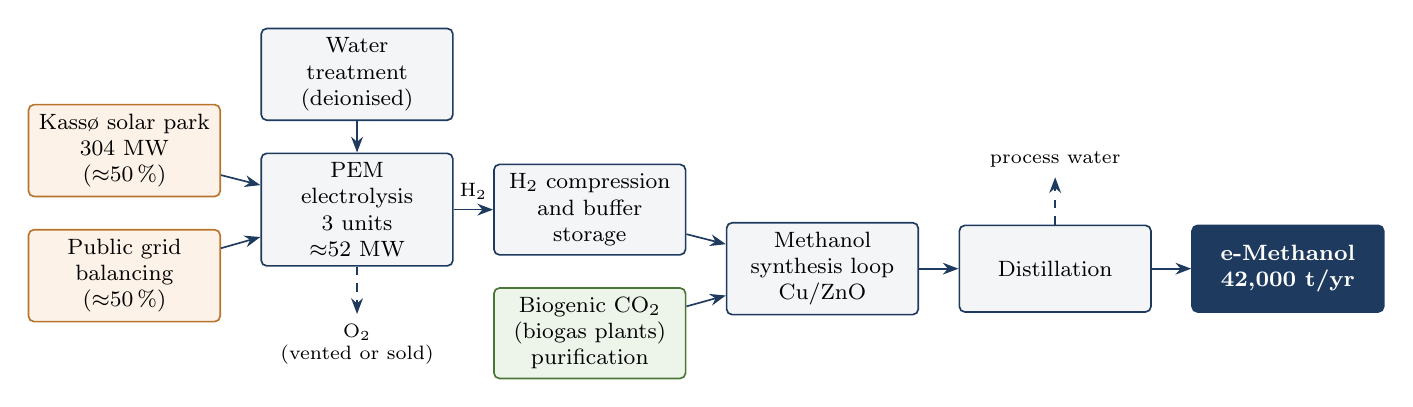
\begin{tikzpicture}[
  node distance=4mm and 5mm,
  box/.style={draw=navy, line width=0.6pt, rounded corners=2pt, fill=navy!5,
              align=center, font=\footnotesize, minimum height=11mm, text width=22mm,
              execute at begin node={\hyphenpenalty=10000}},
  src/.style={box, fill=sun!12, draw=sun!80!black},
  co2/.style={box, fill=leaf!12, draw=leaf!70!black},
  prod/.style={box, fill=navy, text=white, font=\footnotesize\bfseries},
  arr/.style={-{Stealth[length=2mm]}, line width=0.6pt, draw=navy}]
  \node[src] (pv) {Kassø solar park\\304 MW\\($\approx$50\,\%)};
  \node[src, below=of pv] (grid) {Public grid\\balancing\\($\approx$50\,\%)};
  \node[box, right=of pv, yshift=-7.5mm] (el) {PEM electrolysis\\3 units\\$\approx$52 MW};
  \node[box, above=of el] (wt) {Water\\treatment\\(deionised)};
  \node[box, right=of el] (h2) {H$_2$ compression\\and buffer\\storage};
  \node[co2, below=of h2] (co2) {Biogenic CO$_2$\\(biogas plants)\\purification};
  \node[box, right=of h2, yshift=-7.5mm] (syn) {Methanol\\synthesis loop\\Cu/ZnO};
  \node[box, right=of syn] (dist) {Distillation};
  \node[prod, right=of dist] (meoh) {e-Methanol\\42,000 t/yr};
  \draw[arr] (pv) -- (el);
  \draw[arr] (grid) -- (el);
  \draw[arr] (wt) -- (el);
  \draw[arr] (el) -- node[above, font=\scriptsize]{H$_2$} (h2);
  \draw[arr] (h2) -- (syn);
  \draw[arr] (co2) -- (syn);
  \draw[arr] (syn) -- (dist);
  \draw[arr] (dist) -- (meoh);
  \draw[arr, dashed] (el.south) -- ++(0,-6mm) node[below, font=\scriptsize, align=center]{O$_2$\\(vented or sold)};
  \draw[arr, dashed] (dist.north) -- ++(0,6mm) node[above, font=\scriptsize]{process water};
\end{tikzpicture}
\end{document}
